\documentclass[12pt]{article}
\usepackage[breaklinks=true]{hyperref}
\usepackage[margin=0.75in]{geometry}

\usepackage{graphicx}
\usepackage{color}

\definecolor{pblue}{rgb}{0.13,0.13,1}
\definecolor{pgreen}{rgb}{0,0.5,0}
\definecolor{pred}{rgb}{0.9,0,0}
\definecolor{pgrey}{rgb}{0.46,0.45,0.48}

\usepackage{listings}
\lstset{language=Java,
  showspaces=false,
  showtabs=false,
  tabsize=2,
  breaklines=true,
  showstringspaces=false,
  breakatwhitespace=true,
  commentstyle=\color{pgreen},
  keywordstyle=\color{pblue},
  stringstyle=\color{pred},
  basicstyle=\ttfamily,
  frame=single,
  moredelim=[il][\textcolor{pgrey}]{$$},
  moredelim=[is][\textcolor{pgrey}]{\%\%}{\%\%}
}

\title{Concurrency: Writing Multithreaded Programs in Java}
\author{
	Melvyn Ian Drag
}
\date{\today}


\begin{document}
\maketitle

\begin{abstract}
So far the code we've written has been serial - that is to say it does one thing at a time and is oat based. Thanks to fast, multicore CPUs and advanced operating systems, software can be written that performs multiple tasks simultaneously. Concurrency is a very important topic. Tonight you'll learn some basic concepts.
\end{abstract}

\section{Introducion Anecdote}
There is a wide range of computing devices these days. Some of them are simple like these: \textit{indicate an Arduino board}. This little computer is called an Arduino, and it is a fun little device used by children and hobbyists to learn to program. The thing about this computer is that it can only do one thing at a time. The black chip on here \textit{indicate the microcontroller} is an AVR microcontroller. It can only do one operation at a time due to the way that the cpu is designed. To discuss that we'd have to delve into electrical engineering and computer architecture - I'll leave that for you to investigate.

What you usually use is not an Arduino. You usually work with a laptop or desktop, and inside these have big Intel or AMD CPUs.\textit{Go around the class and see if anyone has a Ryzen CPU. Show the class what a CPU looks like if you can find a prop for class.}. These processors have an amazing processing power that you can't even fathom until you start writing high performance code. These processors are likely multiple processors in one. My computer, for example, has a quadcore CPU, which means it actually has 4 processors in one. You can checkout your computer and see what kind of hardware you have.

Now you may ask yourself - why would a computer have more than one processor? It's so that your computer can do multiple things at once! This is something you want. I often open a browser tab and listen to some music on youtube, while checking my email in another window and I probably have a terminal window open too compiling some code. The computer is able to do multiple things at once, like watch youtube, check email, and compile code simultaneously, thanks in part to the multicore architecture of modern CPUs. It's also in part to operating systems being able to schedule multiple tasks. 

Here's an important point: \textbf{Even single core machines with a suitable operating system can give the illusion of multiple operations happening at once.} I don't have a laptop with a single core to demonstrate the concept, but my laptop has a 4 core CPU and it can do more than 4 things at once.



\begin{figure}[h]
  \centering
    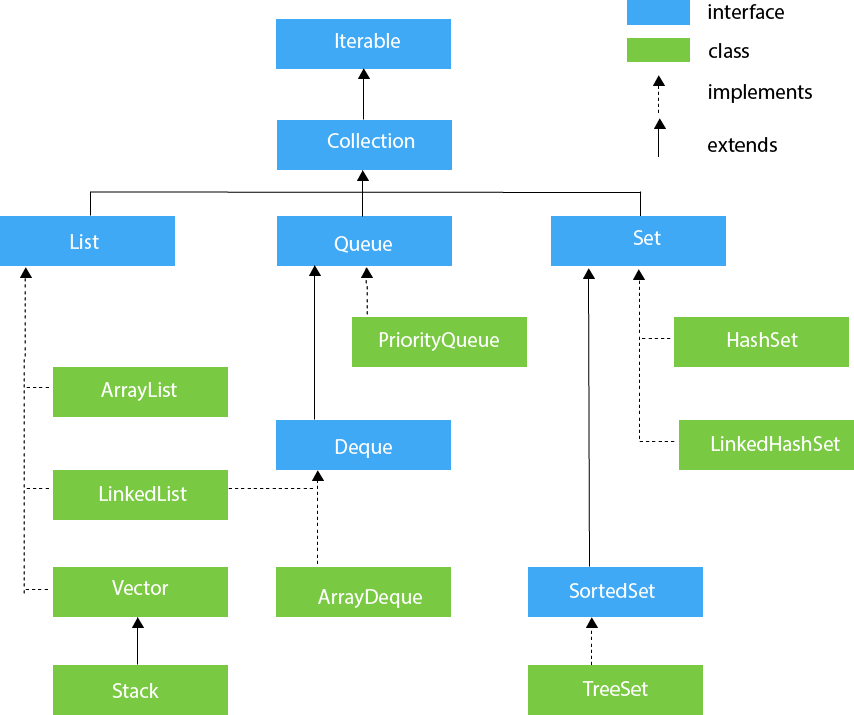
\includegraphics[width=0.5\textwidth]{java-collection-hierarchy.png}
  \caption{Illustration of a variety of classes which implement the Collection class.}
\end{figure}

\end{document}
